\documentclass[1p]{elsarticle_modified}
%\bibliographystyle{elsarticle-num}

%\usepackage[colorlinks]{hyperref}
%\usepackage{abbrmath_seonhwa} %\Abb, \Ascr, \Acal ,\Abf, \Afrak
\usepackage{amsfonts}
\usepackage{amssymb}
\usepackage{amsmath}
\usepackage{amsthm}
\usepackage{scalefnt}
\usepackage{amsbsy}
\usepackage{kotex}
\usepackage{caption}
\usepackage{subfig}
\usepackage{color}
\usepackage{graphicx}
\usepackage{xcolor} %% white, black, red, green, blue, cyan, magenta, yellow
\usepackage{float}
\usepackage{setspace}
\usepackage{hyperref}

\usepackage{tikz}
\usetikzlibrary{arrows}

\usepackage{multirow}
\usepackage{array} % fixed length table
\usepackage{hhline}

%%%%%%%%%%%%%%%%%%%%%
\makeatletter
\renewcommand*\env@matrix[1][\arraystretch]{%
	\edef\arraystretch{#1}%
	\hskip -\arraycolsep
	\let\@ifnextchar\new@ifnextchar
	\array{*\c@MaxMatrixCols c}}
\makeatother %https://tex.stackexchange.com/questions/14071/how-can-i-increase-the-line-spacing-in-a-matrix
%%%%%%%%%%%%%%%

\usepackage[normalem]{ulem}

\newcommand{\msout}[1]{\ifmmode\text{\sout{\ensuremath{#1}}}\else\sout{#1}\fi}
%SOURCE: \msout is \stkout macro in https://tex.stackexchange.com/questions/20609/strikeout-in-math-mode

\newcommand{\cancel}[1]{
	\ifmmode
	{\color{red}\msout{#1}}
	\else
	{\color{red}\sout{#1}}
	\fi
}

\newcommand{\add}[1]{
	{\color{blue}\uwave{#1}}
}

\newcommand{\replace}[2]{
	\ifmmode
	{\color{red}\msout{#1}}{\color{blue}\uwave{#2}}
	\else
	{\color{red}\sout{#1}}{\color{blue}\uwave{#2}}
	\fi
}

\newcommand{\Sol}{\mathcal{S}} %segment
\newcommand{\D}{D} %diagram
\newcommand{\A}{\mathcal{A}} %arc


%%%%%%%%%%%%%%%%%%%%%%%%%%%%%5 test

\def\sl{\operatorname{\textup{SL}}(2,\Cbb)}
\def\psl{\operatorname{\textup{PSL}}(2,\Cbb)}
\def\quan{\mkern 1mu \triangleright \mkern 1mu}

\theoremstyle{definition}
\newtheorem{thm}{Theorem}[section]
\newtheorem{prop}[thm]{Proposition}
\newtheorem{lem}[thm]{Lemma}
\newtheorem{ques}[thm]{Question}
\newtheorem{cor}[thm]{Corollary}
\newtheorem{defn}[thm]{Definition}
\newtheorem{exam}[thm]{Example}
\newtheorem{rmk}[thm]{Remark}
\newtheorem{alg}[thm]{Algorithm}

\newcommand{\I}{\sqrt{-1}}
\begin{document}

%\begin{frontmatter}
%
%\title{Boundary parabolic representations of knots up to 8 crossings}
%
%%% Group authors per affiliation:
%\author{Yunhi Cho} 
%\address{Department of Mathematics, University of Seoul, Seoul, Korea}
%\ead{yhcho@uos.ac.kr}
%
%
%\author{Seonhwa Kim} %\fnref{s_kim}}
%\address{Center for Geometry and Physics, Institute for Basic Science, Pohang, 37673, Korea}
%\ead{ryeona17@ibs.re.kr}
%
%\author{Hyuk Kim}
%\address{Department of Mathematical Sciences, Seoul National University, Seoul 08826, Korea}
%\ead{hyukkim@snu.ac.kr}
%
%\author{Seokbeom Yoon}
%\address{Department of Mathematical Sciences, Seoul National University, Seoul, 08826,  Korea}
%\ead{sbyoon15@snu.ac.kr}
%
%\begin{abstract}
%We find all boundary parabolic representation of knots up to 8 crossings.
%
%\end{abstract}
%\begin{keyword}
%    \MSC[2010] 57M25 
%\end{keyword}
%
%\end{frontmatter}

%\linenumbers
%\tableofcontents
%
\newcommand\colored[1]{\textcolor{white}{\rule[-0.35ex]{0.8em}{1.4ex}}\kern-0.8em\color{red} #1}%
%\newcommand\colored[1]{\textcolor{white}{ #1}\kern-2.17ex	\textcolor{white}{ #1}\kern-1.81ex	\textcolor{white}{ #1}\kern-2.15ex\color{red}#1	}

{\Large $\underline{12n_{0029}~(K12n_{0029})}$}

\setlength{\tabcolsep}{10pt}
\renewcommand{\arraystretch}{1.6}
\vspace{1cm}\begin{tabular}{m{100pt}>{\centering\arraybackslash}m{274pt}}
\multirow{5}{120pt}{
	\centering
	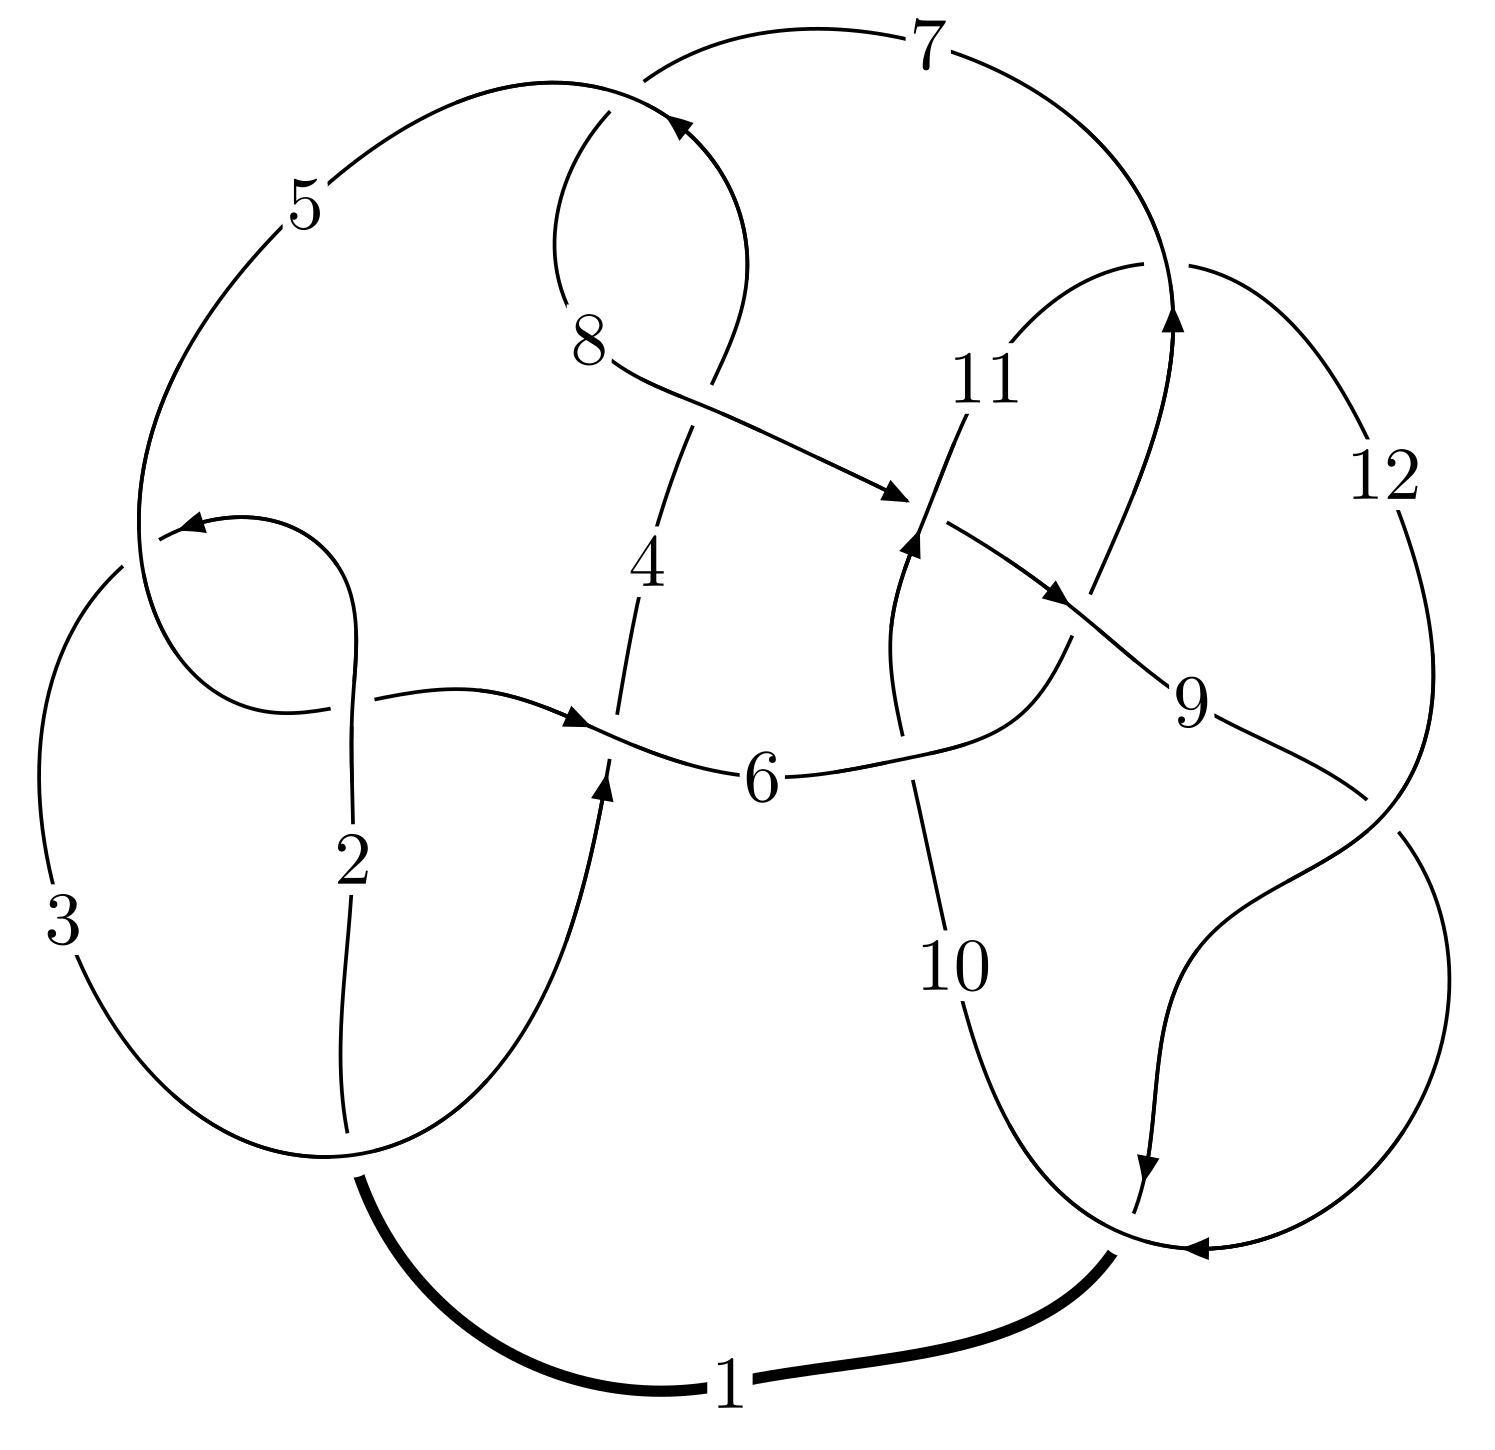
\includegraphics[width=112pt]{../../../GIT/diagram.site/Diagrams/png/2118_12n_0029.png}\\
\ \ \ A knot diagram\footnotemark}&
\allowdisplaybreaks
\textbf{Linearized knot diagam} \\
\cline{2-2}
 &
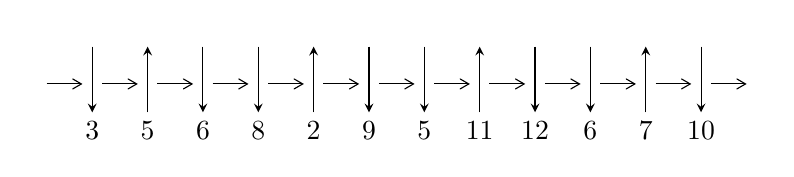
\begin{tikzpicture}[x=20pt, y=17pt]
	% nodes
	\node (C0) at (0, 0) {};
	\node (C1) at (1, 0) {};
	\node (C1U) at (1, +1) {};
	\node (C1D) at (1, -1) {3};

	\node (C2) at (2, 0) {};
	\node (C2U) at (2, +1) {};
	\node (C2D) at (2, -1) {5};

	\node (C3) at (3, 0) {};
	\node (C3U) at (3, +1) {};
	\node (C3D) at (3, -1) {6};

	\node (C4) at (4, 0) {};
	\node (C4U) at (4, +1) {};
	\node (C4D) at (4, -1) {8};

	\node (C5) at (5, 0) {};
	\node (C5U) at (5, +1) {};
	\node (C5D) at (5, -1) {2};

	\node (C6) at (6, 0) {};
	\node (C6U) at (6, +1) {};
	\node (C6D) at (6, -1) {9};

	\node (C7) at (7, 0) {};
	\node (C7U) at (7, +1) {};
	\node (C7D) at (7, -1) {5};

	\node (C8) at (8, 0) {};
	\node (C8U) at (8, +1) {};
	\node (C8D) at (8, -1) {11};

	\node (C9) at (9, 0) {};
	\node (C9U) at (9, +1) {};
	\node (C9D) at (9, -1) {12};

	\node (C10) at (10, 0) {};
	\node (C10U) at (10, +1) {};
	\node (C10D) at (10, -1) {6};

	\node (C11) at (11, 0) {};
	\node (C11U) at (11, +1) {};
	\node (C11D) at (11, -1) {7};

	\node (C12) at (12, 0) {};
	\node (C12U) at (12, +1) {};
	\node (C12D) at (12, -1) {10};
	\node (C13) at (13, 0) {};

	% arrows
	\draw[->,>={angle 60}]
	(C0) edge (C1) (C1) edge (C2) (C2) edge (C3) (C3) edge (C4) (C4) edge (C5) (C5) edge (C6) (C6) edge (C7) (C7) edge (C8) (C8) edge (C9) (C9) edge (C10) (C10) edge (C11) (C11) edge (C12) (C12) edge (C13) ;	\draw[->,>=stealth]
	(C1U) edge (C1D) (C2D) edge (C2U) (C3U) edge (C3D) (C4U) edge (C4D) (C5D) edge (C5U) (C6U) edge (C6D) (C7U) edge (C7D) (C8D) edge (C8U) (C9U) edge (C9D) (C10U) edge (C10D) (C11D) edge (C11U) (C12U) edge (C12D) ;
	\end{tikzpicture} \\
\hhline{~~} \\& 
\textbf{Solving Sequence} \\ \cline{2-2} 
 &
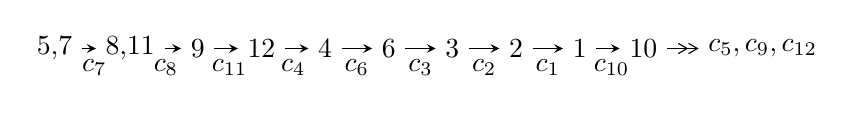
\begin{tikzpicture}[x=23pt, y=7pt]
	% node
	\node (A0) at (-1/8, 0) {5,7};
	\node (A1) at (17/16, 0) {8,11};
	\node (A2) at (17/8, 0) {9};
	\node (A3) at (25/8, 0) {12};
	\node (A4) at (33/8, 0) {4};
	\node (A5) at (41/8, 0) {6};
	\node (A6) at (49/8, 0) {3};
	\node (A7) at (57/8, 0) {2};
	\node (A8) at (65/8, 0) {1};
	\node (A9) at (73/8, 0) {10};
	\node (C1) at (1/2, -1) {$c_{7}$};
	\node (C2) at (13/8, -1) {$c_{8}$};
	\node (C3) at (21/8, -1) {$c_{11}$};
	\node (C4) at (29/8, -1) {$c_{4}$};
	\node (C5) at (37/8, -1) {$c_{6}$};
	\node (C6) at (45/8, -1) {$c_{3}$};
	\node (C7) at (53/8, -1) {$c_{2}$};
	\node (C8) at (61/8, -1) {$c_{1}$};
	\node (C9) at (69/8, -1) {$c_{10}$};
	\node (A10) at (11, 0) {$c_{5},c_{9},c_{12}$};

	% edge
	\draw[->,>=stealth]	
	(A0) edge (A1) (A1) edge (A2) (A2) edge (A3) (A3) edge (A4) (A4) edge (A5) (A5) edge (A6) (A6) edge (A7) (A7) edge (A8) (A8) edge (A9) ;
	\draw[->>,>={angle 60}]	
	(A9) edge (A10);
\end{tikzpicture} \\ 

\end{tabular} \\

\footnotetext{
The image of knot diagram is generated by the software ``\textbf{Draw programme}" developed by Andrew Bartholomew(\url{http://www.layer8.co.uk/maths/draw/index.htm\#Running-draw}), where we modified some parts for our purpose(\url{https://github.com/CATsTAILs/LinksPainter}).
}\phantom \\ \newline 
\centering \textbf{Ideals for irreducible components\footnotemark of $X_{\text{par}}$} 
 
\begin{align*}
I^u_{1}&=\langle 
1.45830\times10^{282} u^{73}-3.06169\times10^{282} u^{72}+\cdots+2.31115\times10^{285} b+2.73476\times10^{285},\\
\phantom{I^u_{1}}&\phantom{= \langle  }1.92674\times10^{282} u^{73}-5.93184\times10^{282} u^{72}+\cdots+1.84892\times10^{285} a-1.31672\times10^{286},\\
\phantom{I^u_{1}}&\phantom{= \langle  }u^{74}-2 u^{73}+\cdots+3072 u+1024\rangle \\
I^u_{2}&=\langle 
u^4-2 u^3- u^2+b+3 u,\;-3 u^4+3 u^3+7 u^2+a-5 u-4,\;u^5- u^4-2 u^3+u^2+u+1\rangle \\
\\
I^v_{1}&=\langle 
a,\;1728 v^9+4936 v^8+9872 v^7-12908 v^6-24680 v^5+34552 v^4+91527 v^3-4936 v^2+3335 b+613,\\
\phantom{I^v_{1}}&\phantom{= \langle  }v^{10}+3 v^9+6 v^8-7 v^7-16 v^6+19 v^5+58 v^4+2 v^3-7 v^2+v+1\rangle \\
\end{align*}
\raggedright * 3 irreducible components of $\dim_{\mathbb{C}}=0$, with total 89 representations.\\
\footnotetext{All coefficients of polynomials are rational numbers. But the coefficients are sometimes approximated in decimal forms when there is not enough margin.}
\newpage
\renewcommand{\arraystretch}{1}
\centering \section*{I. $I^u_{1}= \langle 1.46\times10^{282} u^{73}-3.06\times10^{282} u^{72}+\cdots+2.31\times10^{285} b+2.73\times10^{285},\;1.93\times10^{282} u^{73}-5.93\times10^{282} u^{72}+\cdots+1.85\times10^{285} a-1.32\times10^{286},\;u^{74}-2 u^{73}+\cdots+3072 u+1024 \rangle$}
\flushleft \textbf{(i) Arc colorings}\\
\begin{tabular}{m{7pt} m{180pt} m{7pt} m{180pt} }
\flushright $a_{5}=$&$\begin{pmatrix}0\\u\end{pmatrix}$ \\
\flushright $a_{7}=$&$\begin{pmatrix}1\\0\end{pmatrix}$ \\
\flushright $a_{8}=$&$\begin{pmatrix}1\\u^2\end{pmatrix}$ \\
\flushright $a_{11}=$&$\begin{pmatrix}-0.00104209 u^{73}+0.00320827 u^{72}+\cdots+4.15244 u+7.12158\\-0.000630984 u^{73}+0.00132475 u^{72}+\cdots-3.28645 u-1.18329\end{pmatrix}$ \\
\flushright $a_{9}=$&$\begin{pmatrix}0.000166407 u^{73}-0.0000584423 u^{72}+\cdots-2.97519 u-1.23275\\-0.000372877 u^{73}+0.000687987 u^{72}+\cdots-1.67649 u-0.643683\end{pmatrix}$ \\
\flushright $a_{12}=$&$\begin{pmatrix}-0.00167307 u^{73}+0.00453301 u^{72}+\cdots+0.865989 u+5.93830\\-0.000630984 u^{73}+0.00132475 u^{72}+\cdots-3.28645 u-1.18329\end{pmatrix}$ \\
\flushright $a_{4}=$&$\begin{pmatrix}u\\u^3+u\end{pmatrix}$ \\
\flushright $a_{6}=$&$\begin{pmatrix}-0.0000529417 u^{73}+0.000274782 u^{72}+\cdots+4.64722 u+1.77074\\-0.000269983 u^{73}+0.000677572 u^{72}+\cdots-0.295371 u-0.271861\end{pmatrix}$ \\
\flushright $a_{3}=$&$\begin{pmatrix}0.000525755 u^{73}-0.00116278 u^{72}+\cdots+1.81742 u-0.757111\\-0.0000354351 u^{73}+0.000122315 u^{72}+\cdots+0.573348 u+0.133403\end{pmatrix}$ \\
\flushright $a_{2}=$&$\begin{pmatrix}0.000525755 u^{73}-0.00116278 u^{72}+\cdots+1.81742 u-0.757111\\-0.0000344362 u^{73}+0.0000957799 u^{72}+\cdots+0.376807 u+0.247347\end{pmatrix}$ \\
\flushright $a_{1}=$&$\begin{pmatrix}-0.000150277 u^{73}+0.000195066 u^{72}+\cdots-4.47795 u-1.86965\\-0.000203219 u^{73}+0.000469847 u^{72}+\cdots+0.169272 u-0.0989097\end{pmatrix}$ \\
\flushright $a_{10}=$&$\begin{pmatrix}-0.00137360 u^{73}+0.00403821 u^{72}+\cdots-1.25774 u+5.00923\\-0.000533686 u^{73}+0.00107499 u^{72}+\cdots-2.78713 u-1.04233\end{pmatrix}$\\&\end{tabular}
\flushleft \textbf{(ii) Obstruction class $= -1$}\\~\\
\flushleft \textbf{(iii) Cusp Shapes $= -0.0115164 u^{73}+0.0143583 u^{72}+\cdots-79.5128 u-35.2982$}\\~\\
\newpage\renewcommand{\arraystretch}{1}
\flushleft \textbf{(iv) u-Polynomials at the component}\newline \\
\begin{tabular}{m{50pt}|m{274pt}}
Crossings & \hspace{64pt}u-Polynomials at each crossing \\
\hline $$\begin{aligned}c_{1}\end{aligned}$$&$\begin{aligned}
&u^{74}+23 u^{73}+\cdots-168 u+1
\end{aligned}$\\
\hline $$\begin{aligned}c_{2},c_{5}\end{aligned}$$&$\begin{aligned}
&u^{74}+7 u^{73}+\cdots+10 u+1
\end{aligned}$\\
\hline $$\begin{aligned}c_{3}\end{aligned}$$&$\begin{aligned}
&u^{74}-7 u^{73}+\cdots+23935148 u+1174793
\end{aligned}$\\
\hline $$\begin{aligned}c_{4},c_{7}\end{aligned}$$&$\begin{aligned}
&u^{74}-2 u^{73}+\cdots+3072 u+1024
\end{aligned}$\\
\hline $$\begin{aligned}c_{6}\end{aligned}$$&$\begin{aligned}
&u^{74}-4 u^{73}+\cdots+3 u-1
\end{aligned}$\\
\hline $$\begin{aligned}c_{8}\end{aligned}$$&$\begin{aligned}
&u^{74}+11 u^{73}+\cdots+600 u^2+32
\end{aligned}$\\
\hline $$\begin{aligned}c_{9},c_{12}\end{aligned}$$&$\begin{aligned}
&u^{74}-8 u^{73}+\cdots-83 u-1
\end{aligned}$\\
\hline $$\begin{aligned}c_{10}\end{aligned}$$&$\begin{aligned}
&u^{74}+2 u^{73}+\cdots+140788 u-6632
\end{aligned}$\\
\hline $$\begin{aligned}c_{11}\end{aligned}$$&$\begin{aligned}
&u^{74}-4 u^{73}+\cdots+18563 u+7979
\end{aligned}$\\
\hline
\end{tabular}\\~\\
\newpage\renewcommand{\arraystretch}{1}
\flushleft \textbf{(v) Riley Polynomials at the component}\newline \\
\begin{tabular}{m{50pt}|m{274pt}}
Crossings & \hspace{64pt}Riley Polynomials at each crossing \\
\hline $$\begin{aligned}c_{1}\end{aligned}$$&$\begin{aligned}
&y^{74}+63 y^{73}+\cdots-33884 y+1
\end{aligned}$\\
\hline $$\begin{aligned}c_{2},c_{5}\end{aligned}$$&$\begin{aligned}
&y^{74}+23 y^{73}+\cdots-168 y+1
\end{aligned}$\\
\hline $$\begin{aligned}c_{3}\end{aligned}$$&$\begin{aligned}
&y^{74}+103 y^{73}+\cdots-195612233228368 y+1380138592849
\end{aligned}$\\
\hline $$\begin{aligned}c_{4},c_{7}\end{aligned}$$&$\begin{aligned}
&y^{74}+50 y^{73}+\cdots+5242880 y+1048576
\end{aligned}$\\
\hline $$\begin{aligned}c_{6}\end{aligned}$$&$\begin{aligned}
&y^{74}-20 y^{73}+\cdots+y+1
\end{aligned}$\\
\hline $$\begin{aligned}c_{8}\end{aligned}$$&$\begin{aligned}
&y^{74}-27 y^{73}+\cdots+38400 y+1024
\end{aligned}$\\
\hline $$\begin{aligned}c_{9},c_{12}\end{aligned}$$&$\begin{aligned}
&y^{74}-40 y^{73}+\cdots-2497 y+1
\end{aligned}$\\
\hline $$\begin{aligned}c_{10}\end{aligned}$$&$\begin{aligned}
&y^{74}+78 y^{73}+\cdots-8817552656 y+43983424
\end{aligned}$\\
\hline $$\begin{aligned}c_{11}\end{aligned}$$&$\begin{aligned}
&y^{74}+46 y^{73}+\cdots-1411728345 y+63664441
\end{aligned}$\\
\hline
\end{tabular}\\~\\
\newpage\flushleft \textbf{(vi) Complex Volumes and Cusp Shapes}
$$\begin{array}{c|c|c}  
\text{Solutions to }I^u_{1}& \I (\text{vol} + \sqrt{-1}CS) & \text{Cusp shape}\\
 \hline 
\begin{aligned}
u &= \phantom{-}0.087690 + 1.069920 I \\
a &= -1.70851 + 0.71322 I \\
b &= \phantom{-}0.704260 - 0.483971 I\end{aligned}
 & \phantom{-}0.97521 - 4.62256 I & \phantom{-0.000000 } 0 \\ \hline\begin{aligned}
u &= \phantom{-}0.087690 - 1.069920 I \\
a &= -1.70851 - 0.71322 I \\
b &= \phantom{-}0.704260 + 0.483971 I\end{aligned}
 & \phantom{-}0.97521 + 4.62256 I & \phantom{-0.000000 } 0 \\ \hline\begin{aligned}
u &= \phantom{-}0.384595 + 0.751827 I \\
a &= \phantom{-}0.59893 + 1.37606 I \\
b &= -0.298551 + 0.845553 I\end{aligned}
 & -3.42601 - 3.36523 I & -11.9863 + 8.0764 I \\ \hline\begin{aligned}
u &= \phantom{-}0.384595 - 0.751827 I \\
a &= \phantom{-}0.59893 - 1.37606 I \\
b &= -0.298551 - 0.845553 I\end{aligned}
 & -3.42601 + 3.36523 I & -11.9863 - 8.0764 I \\ \hline\begin{aligned}
u &= \phantom{-}0.495224 + 0.592497 I \\
a &= \phantom{-}2.24773 + 1.14650 I \\
b &= \phantom{-}0.234622 + 0.523186 I\end{aligned}
 & -3.94950 - 0.19450 I & -14.2244 + 0.5338 I \\ \hline\begin{aligned}
u &= \phantom{-}0.495224 - 0.592497 I \\
a &= \phantom{-}2.24773 - 1.14650 I \\
b &= \phantom{-}0.234622 - 0.523186 I\end{aligned}
 & -3.94950 + 0.19450 I & -14.2244 - 0.5338 I \\ \hline\begin{aligned}
u &= \phantom{-}1.247790 + 0.119522 I \\
a &= \phantom{-}0.295580 - 0.114576 I \\
b &= -0.758529 + 0.268504 I\end{aligned}
 & \phantom{-}3.57080 - 3.55900 I & \phantom{-0.000000 } 0 \\ \hline\begin{aligned}
u &= \phantom{-}1.247790 - 0.119522 I \\
a &= \phantom{-}0.295580 + 0.114576 I \\
b &= -0.758529 - 0.268504 I\end{aligned}
 & \phantom{-}3.57080 + 3.55900 I & \phantom{-0.000000 } 0 \\ \hline\begin{aligned}
u &= -0.590376 + 1.132720 I \\
a &= -0.567082 + 0.568941 I \\
b &= \phantom{-}0.416950 + 0.100990 I\end{aligned}
 & -0.18048 + 2.67430 I & \phantom{-0.000000 } 0 \\ \hline\begin{aligned}
u &= -0.590376 - 1.132720 I \\
a &= -0.567082 - 0.568941 I \\
b &= \phantom{-}0.416950 - 0.100990 I\end{aligned}
 & -0.18048 - 2.67430 I & \phantom{-0.000000 } 0\\
 \hline 
 \end{array}$$\newpage$$\begin{array}{c|c|c}  
\text{Solutions to }I^u_{1}& \I (\text{vol} + \sqrt{-1}CS) & \text{Cusp shape}\\
 \hline 
\begin{aligned}
u &= -1.235680 + 0.346795 I \\
a &= \phantom{-}0.250077 + 0.159968 I \\
b &= -0.656348 - 0.079553 I\end{aligned}
 & \phantom{-}3.17540 - 2.27063 I & \phantom{-0.000000 } 0 \\ \hline\begin{aligned}
u &= -1.235680 - 0.346795 I \\
a &= \phantom{-}0.250077 - 0.159968 I \\
b &= -0.656348 + 0.079553 I\end{aligned}
 & \phantom{-}3.17540 + 2.27063 I & \phantom{-0.000000 } 0 \\ \hline\begin{aligned}
u &= \phantom{-}0.100478 + 1.284530 I \\
a &= \phantom{-}1.53887 + 0.10009 I \\
b &= -0.355439 + 0.084862 I\end{aligned}
 & \phantom{-}1.01094 - 2.94591 I & \phantom{-0.000000 } 0 \\ \hline\begin{aligned}
u &= \phantom{-}0.100478 - 1.284530 I \\
a &= \phantom{-}1.53887 - 0.10009 I \\
b &= -0.355439 - 0.084862 I\end{aligned}
 & \phantom{-}1.01094 + 2.94591 I & \phantom{-0.000000 } 0 \\ \hline\begin{aligned}
u &= \phantom{-}0.228131 + 1.295120 I \\
a &= -1.027190 - 0.601335 I \\
b &= \phantom{-}0.757691 + 0.160885 I\end{aligned}
 & \phantom{-}4.23425 + 0.54410 I & \phantom{-0.000000 } 0 \\ \hline\begin{aligned}
u &= \phantom{-}0.228131 - 1.295120 I \\
a &= -1.027190 + 0.601335 I \\
b &= \phantom{-}0.757691 - 0.160885 I\end{aligned}
 & \phantom{-}4.23425 - 0.54410 I & \phantom{-0.000000 } 0 \\ \hline\begin{aligned}
u &= \phantom{-}0.655112 + 0.173687 I \\
a &= \phantom{-}2.35031 + 3.40118 I \\
b &= \phantom{-}0.424294 + 0.991928 I\end{aligned}
 & -1.25518 + 3.58366 I & -11.16812 - 4.57292 I \\ \hline\begin{aligned}
u &= \phantom{-}0.655112 - 0.173687 I \\
a &= \phantom{-}2.35031 - 3.40118 I \\
b &= \phantom{-}0.424294 - 0.991928 I\end{aligned}
 & -1.25518 - 3.58366 I & -11.16812 + 4.57292 I \\ \hline\begin{aligned}
u &= \phantom{-}0.501730 + 0.448793 I \\
a &= \phantom{-}0.554379 - 0.053202 I \\
b &= -0.523151 - 0.840620 I\end{aligned}
 & -0.76340 + 2.05732 I & -6.61172 - 3.28073 I \\ \hline\begin{aligned}
u &= \phantom{-}0.501730 - 0.448793 I \\
a &= \phantom{-}0.554379 + 0.053202 I \\
b &= -0.523151 + 0.840620 I\end{aligned}
 & -0.76340 - 2.05732 I & -6.61172 + 3.28073 I\\
 \hline 
 \end{array}$$\newpage$$\begin{array}{c|c|c}  
\text{Solutions to }I^u_{1}& \I (\text{vol} + \sqrt{-1}CS) & \text{Cusp shape}\\
 \hline 
\begin{aligned}
u &= -0.429078 + 0.495620 I \\
a &= \phantom{-}0.756242 + 0.411909 I \\
b &= \phantom{-}0.048182 - 0.906974 I\end{aligned}
 & -0.75534 + 1.25758 I & -6.16688 - 4.20297 I \\ \hline\begin{aligned}
u &= -0.429078 - 0.495620 I \\
a &= \phantom{-}0.756242 - 0.411909 I \\
b &= \phantom{-}0.048182 + 0.906974 I\end{aligned}
 & -0.75534 - 1.25758 I & -6.16688 + 4.20297 I \\ \hline\begin{aligned}
u &= -0.369003 + 0.540409 I \\
a &= -7.82001 - 3.97910 I \\
b &= -0.53917 + 3.82168 I\end{aligned}
 & -1.96434 + 1.46942 I & \phantom{-}69.4609 + 82.1819 I \\ \hline\begin{aligned}
u &= -0.369003 - 0.540409 I \\
a &= -7.82001 + 3.97910 I \\
b &= -0.53917 - 3.82168 I\end{aligned}
 & -1.96434 - 1.46942 I & \phantom{-}69.4609 - 82.1819 I \\ \hline\begin{aligned}
u &= -0.628002 + 0.177531 I \\
a &= \phantom{-}2.95922 - 3.34855 I \\
b &= \phantom{-}0.457443 - 1.236300 I\end{aligned}
 & -0.94329 + 1.13464 I & -11.14223 - 5.11528 I \\ \hline\begin{aligned}
u &= -0.628002 - 0.177531 I \\
a &= \phantom{-}2.95922 + 3.34855 I \\
b &= \phantom{-}0.457443 + 1.236300 I\end{aligned}
 & -0.94329 - 1.13464 I & -11.14223 + 5.11528 I \\ \hline\begin{aligned}
u &= -0.142745 + 1.346550 I \\
a &= \phantom{-}0.272109 - 0.532528 I \\
b &= -0.260302 - 1.220450 I\end{aligned}
 & \phantom{-}3.14985 + 1.37670 I & \phantom{-0.000000 } 0 \\ \hline\begin{aligned}
u &= -0.142745 - 1.346550 I \\
a &= \phantom{-}0.272109 + 0.532528 I \\
b &= -0.260302 + 1.220450 I\end{aligned}
 & \phantom{-}3.14985 - 1.37670 I & \phantom{-0.000000 } 0 \\ \hline\begin{aligned}
u &= \phantom{-}0.320215 + 1.351930 I \\
a &= \phantom{-}0.198192 + 0.598736 I \\
b &= -0.161270 + 1.198730 I\end{aligned}
 & \phantom{-}2.76643 - 7.39057 I & \phantom{-0.000000 } 0 \\ \hline\begin{aligned}
u &= \phantom{-}0.320215 - 1.351930 I \\
a &= \phantom{-}0.198192 - 0.598736 I \\
b &= -0.161270 - 1.198730 I\end{aligned}
 & \phantom{-}2.76643 + 7.39057 I & \phantom{-0.000000 } 0\\
 \hline 
 \end{array}$$\newpage$$\begin{array}{c|c|c}  
\text{Solutions to }I^u_{1}& \I (\text{vol} + \sqrt{-1}CS) & \text{Cusp shape}\\
 \hline 
\begin{aligned}
u &= -0.173717 + 0.574494 I \\
a &= \phantom{-}1.239130 + 0.100705 I \\
b &= -0.321576 - 1.059120 I\end{aligned}
 & -0.71671 + 1.37236 I & -4.04860 - 4.25236 I \\ \hline\begin{aligned}
u &= -0.173717 - 0.574494 I \\
a &= \phantom{-}1.239130 - 0.100705 I \\
b &= -0.321576 + 1.059120 I\end{aligned}
 & -0.71671 - 1.37236 I & -4.04860 + 4.25236 I \\ \hline\begin{aligned}
u &= -0.298851 + 0.519319 I \\
a &= \phantom{-}1.328640 + 0.298136 I \\
b &= -0.182893 - 0.326086 I\end{aligned}
 & -0.31180 + 1.54577 I & -2.35841 - 4.98495 I \\ \hline\begin{aligned}
u &= -0.298851 - 0.519319 I \\
a &= \phantom{-}1.328640 - 0.298136 I \\
b &= -0.182893 + 0.326086 I\end{aligned}
 & -0.31180 - 1.54577 I & -2.35841 + 4.98495 I \\ \hline\begin{aligned}
u &= \phantom{-}0.490220 + 0.320949 I \\
a &= \phantom{-}0.0858483 + 0.0914575 I \\
b &= \phantom{-}0.568197 + 1.214540 I\end{aligned}
 & -6.11124 + 6.05756 I & -13.16929 + 2.49659 I \\ \hline\begin{aligned}
u &= \phantom{-}0.490220 - 0.320949 I \\
a &= \phantom{-}0.0858483 - 0.0914575 I \\
b &= \phantom{-}0.568197 - 1.214540 I\end{aligned}
 & -6.11124 - 6.05756 I & -13.16929 - 2.49659 I \\ \hline\begin{aligned}
u &= -0.425333 + 0.359403 I \\
a &= \phantom{-}0.0853519 + 0.0910101 I \\
b &= \phantom{-}0.371695 + 1.137080 I\end{aligned}
 & -5.95413 + 2.77149 I & -11.1970 - 11.7984 I \\ \hline\begin{aligned}
u &= -0.425333 - 0.359403 I \\
a &= \phantom{-}0.0853519 - 0.0910101 I \\
b &= \phantom{-}0.371695 - 1.137080 I\end{aligned}
 & -5.95413 - 2.77149 I & -11.1970 + 11.7984 I \\ \hline\begin{aligned}
u &= -1.44330\phantom{ +0.000000I} \\
a &= \phantom{-}0.133015\phantom{ +0.000000I} \\
b &= \phantom{-}0.809332\phantom{ +0.000000I}\end{aligned}
 & -3.60099\phantom{ +0.000000I} & \phantom{-0.000000 } 0 \\ \hline\begin{aligned}
u &= \phantom{-}0.01717 + 1.45367 I \\
a &= -0.539494 + 0.887846 I \\
b &= \phantom{-}0.66032 - 2.68740 I\end{aligned}
 & \phantom{-}4.88888 + 2.03616 I & \phantom{-0.000000 } 0\\
 \hline 
 \end{array}$$\newpage$$\begin{array}{c|c|c}  
\text{Solutions to }I^u_{1}& \I (\text{vol} + \sqrt{-1}CS) & \text{Cusp shape}\\
 \hline 
\begin{aligned}
u &= \phantom{-}0.01717 - 1.45367 I \\
a &= -0.539494 - 0.887846 I \\
b &= \phantom{-}0.66032 + 2.68740 I\end{aligned}
 & \phantom{-}4.88888 - 2.03616 I & \phantom{-0.000000 } 0 \\ \hline\begin{aligned}
u &= -0.20391 + 1.44776 I \\
a &= -0.773494 - 0.847749 I \\
b &= \phantom{-}0.54517 + 2.88900 I\end{aligned}
 & \phantom{-}4.71109 + 4.13291 I & \phantom{-0.000000 } 0 \\ \hline\begin{aligned}
u &= -0.20391 - 1.44776 I \\
a &= -0.773494 + 0.847749 I \\
b &= \phantom{-}0.54517 - 2.88900 I\end{aligned}
 & \phantom{-}4.71109 - 4.13291 I & \phantom{-0.000000 } 0 \\ \hline\begin{aligned}
u &= \phantom{-}0.44904 + 1.39545 I \\
a &= \phantom{-}1.389400 - 0.053483 I \\
b &= -1.19431 + 1.06464 I\end{aligned}
 & -1.87183 - 10.09290 I & \phantom{-0.000000 } 0 \\ \hline\begin{aligned}
u &= \phantom{-}0.44904 - 1.39545 I \\
a &= \phantom{-}1.389400 + 0.053483 I \\
b &= -1.19431 - 1.06464 I\end{aligned}
 & -1.87183 + 10.09290 I & \phantom{-0.000000 } 0 \\ \hline\begin{aligned}
u &= \phantom{-}0.08788 + 1.46777 I \\
a &= \phantom{-}1.035950 - 0.323500 I \\
b &= -1.179080 + 0.604061 I\end{aligned}
 & -0.83764 - 1.21344 I & \phantom{-0.000000 } 0 \\ \hline\begin{aligned}
u &= \phantom{-}0.08788 - 1.46777 I \\
a &= \phantom{-}1.035950 + 0.323500 I \\
b &= -1.179080 - 0.604061 I\end{aligned}
 & -0.83764 + 1.21344 I & \phantom{-0.000000 } 0 \\ \hline\begin{aligned}
u &= \phantom{-}1.48809 + 0.13110 I \\
a &= \phantom{-}0.0912489 - 0.0358039 I \\
b &= \phantom{-}0.598953 - 0.223005 I\end{aligned}
 & -7.41606 - 4.57419 I & \phantom{-0.000000 } 0 \\ \hline\begin{aligned}
u &= \phantom{-}1.48809 - 0.13110 I \\
a &= \phantom{-}0.0912489 + 0.0358039 I \\
b &= \phantom{-}0.598953 + 0.223005 I\end{aligned}
 & -7.41606 + 4.57419 I & \phantom{-0.000000 } 0 \\ \hline\begin{aligned}
u &= \phantom{-}0.125495 + 0.432831 I \\
a &= \phantom{-}7.30187 + 2.79699 I \\
b &= -1.075840 + 0.578988 I\end{aligned}
 & -2.18804 + 1.82733 I & \phantom{-}11.01430 - 3.60905 I\\
 \hline 
 \end{array}$$\newpage$$\begin{array}{c|c|c}  
\text{Solutions to }I^u_{1}& \I (\text{vol} + \sqrt{-1}CS) & \text{Cusp shape}\\
 \hline 
\begin{aligned}
u &= \phantom{-}0.125495 - 0.432831 I \\
a &= \phantom{-}7.30187 - 2.79699 I \\
b &= -1.075840 - 0.578988 I\end{aligned}
 & -2.18804 - 1.82733 I & \phantom{-}11.01430 + 3.60905 I \\ \hline\begin{aligned}
u &= \phantom{-}1.52778 + 0.35064 I \\
a &= \phantom{-}0.095478 + 0.108395 I \\
b &= \phantom{-}1.31875 + 0.93719 I\end{aligned}
 & \phantom{-}1.67555 + 9.13934 I & \phantom{-0.000000 } 0 \\ \hline\begin{aligned}
u &= \phantom{-}1.52778 - 0.35064 I \\
a &= \phantom{-}0.095478 - 0.108395 I \\
b &= \phantom{-}1.31875 - 0.93719 I\end{aligned}
 & \phantom{-}1.67555 - 9.13934 I & \phantom{-0.000000 } 0 \\ \hline\begin{aligned}
u &= -1.55967 + 0.19709 I \\
a &= \phantom{-}0.104540 - 0.110896 I \\
b &= \phantom{-}1.33678 - 0.74411 I\end{aligned}
 & \phantom{-}2.10183 - 2.80934 I & \phantom{-0.000000 } 0 \\ \hline\begin{aligned}
u &= -1.55967 - 0.19709 I \\
a &= \phantom{-}0.104540 + 0.110896 I \\
b &= \phantom{-}1.33678 + 0.74411 I\end{aligned}
 & \phantom{-}2.10183 + 2.80934 I & \phantom{-0.000000 } 0 \\ \hline\begin{aligned}
u &= -0.27655 + 1.57965 I \\
a &= \phantom{-}1.126550 + 0.143036 I \\
b &= -1.37108 - 0.84338 I\end{aligned}
 & \phantom{-}2.84481 + 6.06997 I & \phantom{-0.000000 } 0 \\ \hline\begin{aligned}
u &= -0.27655 - 1.57965 I \\
a &= \phantom{-}1.126550 - 0.143036 I \\
b &= -1.37108 + 0.84338 I\end{aligned}
 & \phantom{-}2.84481 - 6.06997 I & \phantom{-0.000000 } 0 \\ \hline\begin{aligned}
u &= -0.81564 + 1.38136 I \\
a &= -0.753914 + 0.369227 I \\
b &= \phantom{-}0.663812 + 0.540105 I\end{aligned}
 & \phantom{-}6.17331 + 9.63827 I & \phantom{-0.000000 } 0 \\ \hline\begin{aligned}
u &= -0.81564 - 1.38136 I \\
a &= -0.753914 - 0.369227 I \\
b &= \phantom{-}0.663812 - 0.540105 I\end{aligned}
 & \phantom{-}6.17331 - 9.63827 I & \phantom{-0.000000 } 0 \\ \hline\begin{aligned}
u &= \phantom{-}0.72899 + 1.43535 I \\
a &= -0.757398 - 0.390640 I \\
b &= \phantom{-}0.743568 - 0.424934 I\end{aligned}
 & \phantom{-}7.41718 - 3.39847 I & \phantom{-0.000000 } 0\\
 \hline 
 \end{array}$$\newpage$$\begin{array}{c|c|c}  
\text{Solutions to }I^u_{1}& \I (\text{vol} + \sqrt{-1}CS) & \text{Cusp shape}\\
 \hline 
\begin{aligned}
u &= \phantom{-}0.72899 - 1.43535 I \\
a &= -0.757398 + 0.390640 I \\
b &= \phantom{-}0.743568 + 0.424934 I\end{aligned}
 & \phantom{-}7.41718 + 3.39847 I & \phantom{-0.000000 } 0 \\ \hline\begin{aligned}
u &= \phantom{-}0.53611 + 1.52849 I \\
a &= -1.274840 - 0.153132 I \\
b &= \phantom{-}1.123730 - 0.679779 I\end{aligned}
 & \phantom{-}8.83947 - 10.02070 I & \phantom{-0.000000 } 0 \\ \hline\begin{aligned}
u &= \phantom{-}0.53611 - 1.52849 I \\
a &= -1.274840 + 0.153132 I \\
b &= \phantom{-}1.123730 + 0.679779 I\end{aligned}
 & \phantom{-}8.83947 + 10.02070 I & \phantom{-0.000000 } 0 \\ \hline\begin{aligned}
u &= -0.39620 + 1.58131 I \\
a &= -1.232710 + 0.026127 I \\
b &= \phantom{-}1.138660 + 0.572588 I\end{aligned}
 & \phantom{-}9.56303 + 3.64207 I & \phantom{-0.000000 } 0 \\ \hline\begin{aligned}
u &= -0.39620 - 1.58131 I \\
a &= -1.232710 - 0.026127 I \\
b &= \phantom{-}1.138660 - 0.572588 I\end{aligned}
 & \phantom{-}9.56303 - 3.64207 I & \phantom{-0.000000 } 0 \\ \hline\begin{aligned}
u &= \phantom{-}0.81404 + 1.47762 I \\
a &= \phantom{-}1.239280 + 0.352565 I \\
b &= -1.30347 + 1.39965 I\end{aligned}
 & \phantom{-}5.3004 - 17.3091 I & \phantom{-0.000000 } 0 \\ \hline\begin{aligned}
u &= \phantom{-}0.81404 - 1.47762 I \\
a &= \phantom{-}1.239280 - 0.352565 I \\
b &= -1.30347 - 1.39965 I\end{aligned}
 & \phantom{-}5.3004 + 17.3091 I & \phantom{-0.000000 } 0 \\ \hline\begin{aligned}
u &= -0.73726 + 1.55967 I \\
a &= \phantom{-}1.195100 - 0.255132 I \\
b &= -1.37771 - 1.32852 I\end{aligned}
 & \phantom{-}6.50731 + 10.89880 I & \phantom{-0.000000 } 0 \\ \hline\begin{aligned}
u &= -0.73726 - 1.55967 I \\
a &= \phantom{-}1.195100 + 0.255132 I \\
b &= -1.37771 + 1.32852 I\end{aligned}
 & \phantom{-}6.50731 - 10.89880 I & \phantom{-0.000000 } 0 \\ \hline\begin{aligned}
u &= -0.272195\phantom{ +0.000000I} \\
a &= \phantom{-}4.54371\phantom{ +0.000000I} \\
b &= \phantom{-}0.970995\phantom{ +0.000000I}\end{aligned}
 & -2.30896\phantom{ +0.000000I} & -2.48640\phantom{ +0.000000I}\\
 \hline 
 \end{array}$$\newpage$$\begin{array}{c|c|c}  
\text{Solutions to }I^u_{1}& \I (\text{vol} + \sqrt{-1}CS) & \text{Cusp shape}\\
 \hline 
\begin{aligned}
u &= -0.45730 + 1.67049 I \\
a &= \phantom{-}0.889473 - 0.300191 I \\
b &= -1.71368 - 0.14443 I\end{aligned}
 & \phantom{-}8.61435 + 4.58115 I & \phantom{-0.000000 } 0 \\ \hline\begin{aligned}
u &= -0.45730 - 1.67049 I \\
a &= \phantom{-}0.889473 + 0.300191 I \\
b &= -1.71368 + 0.14443 I\end{aligned}
 & \phantom{-}8.61435 - 4.58115 I & \phantom{-0.000000 } 0 \\ \hline\begin{aligned}
u &= \phantom{-}0.31130 + 1.74570 I \\
a &= \phantom{-}0.886783 + 0.250968 I \\
b &= -1.73082 - 0.07312 I\end{aligned}
 & \phantom{-}9.18515 + 2.01287 I & \phantom{-0.000000 } 0 \\ \hline\begin{aligned}
u &= \phantom{-}0.31130 - 1.74570 I \\
a &= \phantom{-}0.886783 - 0.250968 I \\
b &= -1.73082 + 0.07312 I\end{aligned}
 & \phantom{-}9.18515 - 2.01287 I & \phantom{-0.000000 } 0\\
 \hline 
 \end{array}$$\newpage\newpage\renewcommand{\arraystretch}{1}
\centering \section*{II. $I^u_{2}= \langle u^4-2 u^3- u^2+b+3 u,\;-3 u^4+3 u^3+7 u^2+a-5 u-4,\;u^5- u^4-2 u^3+u^2+u+1 \rangle$}
\flushleft \textbf{(i) Arc colorings}\\
\begin{tabular}{m{7pt} m{180pt} m{7pt} m{180pt} }
\flushright $a_{5}=$&$\begin{pmatrix}0\\u\end{pmatrix}$ \\
\flushright $a_{7}=$&$\begin{pmatrix}1\\0\end{pmatrix}$ \\
\flushright $a_{8}=$&$\begin{pmatrix}1\\u^2\end{pmatrix}$ \\
\flushright $a_{11}=$&$\begin{pmatrix}3 u^4-3 u^3-7 u^2+5 u+4\\- u^4+2 u^3+u^2-3 u\end{pmatrix}$ \\
\flushright $a_{9}=$&$\begin{pmatrix}1\\u^2\end{pmatrix}$ \\
\flushright $a_{12}=$&$\begin{pmatrix}2 u^4- u^3-6 u^2+2 u+4\\- u^4+2 u^3+u^2-3 u\end{pmatrix}$ \\
\flushright $a_{4}=$&$\begin{pmatrix}u\\u^3+u\end{pmatrix}$ \\
\flushright $a_{6}=$&$\begin{pmatrix}- u^2+1\\- u^4\end{pmatrix}$ \\
\flushright $a_{3}=$&$\begin{pmatrix}- u^3+2 u\\- u^4- u^3+u^2+2 u+1\end{pmatrix}$ \\
\flushright $a_{2}=$&$\begin{pmatrix}- u^3+2 u\\-2 u^4- u^3+2 u^2+3 u+2\end{pmatrix}$ \\
\flushright $a_{1}=$&$\begin{pmatrix}-1\\- u^2\end{pmatrix}$ \\
\flushright $a_{10}=$&$\begin{pmatrix}2 u^4- u^3-6 u^2+2 u+5\\- u^4+2 u^3+2 u^2-3 u\end{pmatrix}$\\&\end{tabular}
\flushleft \textbf{(ii) Obstruction class $= 1$}\\~\\
\flushleft \textbf{(iii) Cusp Shapes $= -24 u^4+29 u^3+27 u^2-44 u-1$}\\~\\
\newpage\renewcommand{\arraystretch}{1}
\flushleft \textbf{(iv) u-Polynomials at the component}\newline \\
\begin{tabular}{m{50pt}|m{274pt}}
Crossings & \hspace{64pt}u-Polynomials at each crossing \\
\hline $$\begin{aligned}c_{1}\end{aligned}$$&$\begin{aligned}
&u^5-3 u^4+4 u^3- u^2- u+1
\end{aligned}$\\
\hline $$\begin{aligned}c_{2}\end{aligned}$$&$\begin{aligned}
&u^5- u^4+2 u^3- u^2+u-1
\end{aligned}$\\
\hline $$\begin{aligned}c_{3},c_{4}\end{aligned}$$&$\begin{aligned}
&u^5+u^4-2 u^3- u^2+u-1
\end{aligned}$\\
\hline $$\begin{aligned}c_{5}\end{aligned}$$&$\begin{aligned}
&u^5+u^4+2 u^3+u^2+u+1
\end{aligned}$\\
\hline $$\begin{aligned}c_{6}\end{aligned}$$&$\begin{aligned}
&u^5-5 u^4+8 u^3-3 u^2- u-1
\end{aligned}$\\
\hline $$\begin{aligned}c_{7}\end{aligned}$$&$\begin{aligned}
&u^5- u^4-2 u^3+u^2+u+1
\end{aligned}$\\
\hline $$\begin{aligned}c_{8}\end{aligned}$$&$\begin{aligned}
&u^5
\end{aligned}$\\
\hline $$\begin{aligned}c_{9}\end{aligned}$$&$\begin{aligned}
&(u-1)^5
\end{aligned}$\\
\hline $$\begin{aligned}c_{10},c_{11}\end{aligned}$$&$\begin{aligned}
&u^5+u^4+3 u^3-8 u^2+5 u-1
\end{aligned}$\\
\hline $$\begin{aligned}c_{12}\end{aligned}$$&$\begin{aligned}
&(u+1)^5
\end{aligned}$\\
\hline
\end{tabular}\\~\\
\newpage\renewcommand{\arraystretch}{1}
\flushleft \textbf{(v) Riley Polynomials at the component}\newline \\
\begin{tabular}{m{50pt}|m{274pt}}
Crossings & \hspace{64pt}Riley Polynomials at each crossing \\
\hline $$\begin{aligned}c_{1}\end{aligned}$$&$\begin{aligned}
&y^5- y^4+8 y^3-3 y^2+3 y-1
\end{aligned}$\\
\hline $$\begin{aligned}c_{2},c_{5}\end{aligned}$$&$\begin{aligned}
&y^5+3 y^4+4 y^3+y^2- y-1
\end{aligned}$\\
\hline $$\begin{aligned}c_{3},c_{4},c_{7}\end{aligned}$$&$\begin{aligned}
&y^5-5 y^4+8 y^3-3 y^2- y-1
\end{aligned}$\\
\hline $$\begin{aligned}c_{6}\end{aligned}$$&$\begin{aligned}
&y^5-9 y^4+32 y^3-35 y^2-5 y-1
\end{aligned}$\\
\hline $$\begin{aligned}c_{8}\end{aligned}$$&$\begin{aligned}
&y^5
\end{aligned}$\\
\hline $$\begin{aligned}c_{9},c_{12}\end{aligned}$$&$\begin{aligned}
&(y-1)^5
\end{aligned}$\\
\hline $$\begin{aligned}c_{10},c_{11}\end{aligned}$$&$\begin{aligned}
&y^5+5 y^4+35 y^3-32 y^2+9 y-1
\end{aligned}$\\
\hline
\end{tabular}\\~\\
\newpage\flushleft \textbf{(vi) Complex Volumes and Cusp Shapes}
$$\begin{array}{c|c|c}  
\text{Solutions to }I^u_{2}& \I (\text{vol} + \sqrt{-1}CS) & \text{Cusp shape}\\
 \hline 
\begin{aligned}
u &= -1.21774\phantom{ +0.000000I} \\
a &= -0.454765\phantom{ +0.000000I} \\
b &= -0.674363\phantom{ +0.000000I}\end{aligned}
 & -4.04602\phantom{ +0.000000I} & -12.5230\phantom{ +0.000000I} \\ \hline\begin{aligned}
u &= -0.309916 + 0.549911 I \\
a &= \phantom{-}2.91994 + 5.58105 I \\
b &= \phantom{-}1.29977 - 2.14694 I\end{aligned}
 & -1.97403 + 1.53058 I & \phantom{-}16.1214 - 37.0026 I \\ \hline\begin{aligned}
u &= -0.309916 - 0.549911 I \\
a &= \phantom{-}2.91994 - 5.58105 I \\
b &= \phantom{-}1.29977 + 2.14694 I\end{aligned}
 & -1.97403 - 1.53058 I & \phantom{-}16.1214 + 37.0026 I \\ \hline\begin{aligned}
u &= \phantom{-}1.41878 + 0.21917 I \\
a &= -0.192553 + 0.135455 I \\
b &= -0.462589 + 0.146410 I\end{aligned}
 & -7.51750 - 4.40083 I & -16.8598 - 13.4304 I \\ \hline\begin{aligned}
u &= \phantom{-}1.41878 - 0.21917 I \\
a &= -0.192553 - 0.135455 I \\
b &= -0.462589 - 0.146410 I\end{aligned}
 & -7.51750 + 4.40083 I & -16.8598 + 13.4304 I\\
 \hline 
 \end{array}$$\newpage\newpage\renewcommand{\arraystretch}{1}
\centering \section*{III. $I^v_{1}= \langle a,\;1728 v^9+4936 v^8+\cdots+3335 b+613,\;v^{10}+3 v^9+\cdots+v+1 \rangle$}
\flushleft \textbf{(i) Arc colorings}\\
\begin{tabular}{m{7pt} m{180pt} m{7pt} m{180pt} }
\flushright $a_{5}=$&$\begin{pmatrix}v\\0\end{pmatrix}$ \\
\flushright $a_{7}=$&$\begin{pmatrix}1\\0\end{pmatrix}$ \\
\flushright $a_{8}=$&$\begin{pmatrix}1\\0\end{pmatrix}$ \\
\flushright $a_{11}=$&$\begin{pmatrix}0\\-0.518141 v^{9}-1.48006 v^{8}+\cdots+1.48006 v^{2}-0.183808\end{pmatrix}$ \\
\flushright $a_{9}=$&$\begin{pmatrix}1\\0.462969 v^{9}+1.33373 v^{8}+\cdots-1.33373 v^{2}+1.81379\end{pmatrix}$ \\
\flushright $a_{12}=$&$\begin{pmatrix}-0.518141 v^{9}-1.48006 v^{8}+\cdots+1.48006 v^{2}-0.183808\\-0.518141 v^{9}-1.48006 v^{8}+\cdots+1.48006 v^{2}-0.183808\end{pmatrix}$ \\
\flushright $a_{4}=$&$\begin{pmatrix}v\\0\end{pmatrix}$ \\
\flushright $a_{6}=$&$\begin{pmatrix}-0.462969 v^{9}-1.33373 v^{8}+\cdots+1.33373 v^{2}-0.813793\\-1.14783 v^{9}-3.29565 v^{8}+\cdots+3.29565 v^{2}-1.75652\end{pmatrix}$ \\
\flushright $a_{3}=$&$\begin{pmatrix}0.0740630 v^{9}+0.148126 v^{8}+\cdots+3.77811 v+0.424888\\0.147826 v^{9}+0.295652 v^{8}+\cdots+7 v+0.756522\end{pmatrix}$ \\
\flushright $a_{2}=$&$\begin{pmatrix}-0.0737631 v^{9}-0.277961 v^{8}+\cdots+3.77811 v+0.277061\\0.147826 v^{9}+0.295652 v^{8}+\cdots+7 v+0.756522\end{pmatrix}$ \\
\flushright $a_{1}=$&$\begin{pmatrix}0.462969 v^{9}+1.33373 v^{8}+\cdots-1.33373 v^{2}+0.813793\\1.14783 v^{9}+3.29565 v^{8}+\cdots-3.29565 v^{2}+1.75652\end{pmatrix}$ \\
\flushright $a_{10}=$&$\begin{pmatrix}0.684858 v^{9}+1.96192 v^{8}+\cdots-1.96192 v^{2}+0.942729\\1.14783 v^{9}+3.29565 v^{8}+\cdots-3.29565 v^{2}+1.75652\end{pmatrix}$\\&\end{tabular}
\flushleft \textbf{(ii) Obstruction class $= 1$}\\~\\
\flushleft \textbf{(iii) Cusp Shapes $= \frac{10239}{3335} v^9+\frac{24678}{3335} v^8+\frac{44281}{3335} v^7-\frac{105719}{3335} v^6-\frac{23431}{667} v^5+\frac{281061}{3335} v^4+\frac{471061}{3335} v^3-\frac{304673}{3335} v^2-\frac{263}{23} v+\frac{12334}{3335}$}\\~\\
\newpage\renewcommand{\arraystretch}{1}
\flushleft \textbf{(iv) u-Polynomials at the component}\newline \\
\begin{tabular}{m{50pt}|m{274pt}}
Crossings & \hspace{64pt}u-Polynomials at each crossing \\
\hline $$\begin{aligned}c_{1},c_{3},c_{5}\end{aligned}$$&$\begin{aligned}
&(u^2- u+1)^5
\end{aligned}$\\
\hline $$\begin{aligned}c_{2}\end{aligned}$$&$\begin{aligned}
&(u^2+u+1)^5
\end{aligned}$\\
\hline $$\begin{aligned}c_{4},c_{7}\end{aligned}$$&$\begin{aligned}
&u^{10}
\end{aligned}$\\
\hline $$\begin{aligned}c_{6}\end{aligned}$$&$\begin{aligned}
&(u^5-3 u^4+4 u^3- u^2- u+1)^2
\end{aligned}$\\
\hline $$\begin{aligned}c_{8}\end{aligned}$$&$\begin{aligned}
&(u^5- u^4+2 u^3- u^2+u-1)^2
\end{aligned}$\\
\hline $$\begin{aligned}c_{9}\end{aligned}$$&$\begin{aligned}
&(u^5+u^4-2 u^3- u^2+u-1)^2
\end{aligned}$\\
\hline $$\begin{aligned}c_{10},c_{12}\end{aligned}$$&$\begin{aligned}
&(u^5- u^4-2 u^3+u^2+u+1)^2
\end{aligned}$\\
\hline $$\begin{aligned}c_{11}\end{aligned}$$&$\begin{aligned}
&(u^5+u^4+2 u^3+u^2+u+1)^2
\end{aligned}$\\
\hline
\end{tabular}\\~\\
\newpage\renewcommand{\arraystretch}{1}
\flushleft \textbf{(v) Riley Polynomials at the component}\newline \\
\begin{tabular}{m{50pt}|m{274pt}}
Crossings & \hspace{64pt}Riley Polynomials at each crossing \\
\hline $$\begin{aligned}c_{1},c_{2},c_{3}\\c_{5}\end{aligned}$$&$\begin{aligned}
&(y^2+y+1)^5
\end{aligned}$\\
\hline $$\begin{aligned}c_{4},c_{7}\end{aligned}$$&$\begin{aligned}
&y^{10}
\end{aligned}$\\
\hline $$\begin{aligned}c_{6}\end{aligned}$$&$\begin{aligned}
&(y^5- y^4+8 y^3-3 y^2+3 y-1)^2
\end{aligned}$\\
\hline $$\begin{aligned}c_{8},c_{11}\end{aligned}$$&$\begin{aligned}
&(y^5+3 y^4+4 y^3+y^2- y-1)^2
\end{aligned}$\\
\hline $$\begin{aligned}c_{9},c_{10},c_{12}\end{aligned}$$&$\begin{aligned}
&(y^5-5 y^4+8 y^3-3 y^2- y-1)^2
\end{aligned}$\\
\hline
\end{tabular}\\~\\
\newpage\flushleft \textbf{(vi) Complex Volumes and Cusp Shapes}
$$\begin{array}{c|c|c}  
\text{Solutions to }I^v_{1}& \I (\text{vol} + \sqrt{-1}CS) & \text{Cusp shape}\\
 \hline 
\begin{aligned}
v &= -1.38814 + 0.78973 I \\
a &= \phantom{-0.000000 } 0 \\
b &= -0.339110 + 0.822375 I\end{aligned}
 & -0.32910 - 3.56046 I & -3.01153 + 6.03927 I \\ \hline\begin{aligned}
v &= -1.38814 - 0.78973 I \\
a &= \phantom{-0.000000 } 0 \\
b &= -0.339110 - 0.822375 I\end{aligned}
 & -0.32910 + 3.56046 I & -3.01153 - 6.03927 I \\ \hline\begin{aligned}
v &= \phantom{-}1.37799 + 0.80730 I \\
a &= \phantom{-0.000000 } 0 \\
b &= -0.339110 + 0.822375 I\end{aligned}
 & -0.329100 + 0.499304 I & -3.07628 + 2.84945 I \\ \hline\begin{aligned}
v &= \phantom{-}1.37799 - 0.80730 I \\
a &= \phantom{-0.000000 } 0 \\
b &= -0.339110 - 0.822375 I\end{aligned}
 & -0.329100 - 0.499304 I & -3.07628 - 2.84945 I \\ \hline\begin{aligned}
v &= \phantom{-}0.294694 + 0.220725 I \\
a &= \phantom{-0.000000 } 0 \\
b &= \phantom{-}0.455697 - 1.200150 I\end{aligned}
 & -5.87256 - 2.37095 I & -6.63163 - 6.91428 I \\ \hline\begin{aligned}
v &= \phantom{-}0.294694 - 0.220725 I \\
a &= \phantom{-0.000000 } 0 \\
b &= \phantom{-}0.455697 + 1.200150 I\end{aligned}
 & -5.87256 + 2.37095 I & -6.63163 + 6.91428 I \\ \hline\begin{aligned}
v &= -0.338500 + 0.144851 I \\
a &= \phantom{-0.000000 } 0 \\
b &= \phantom{-}0.455697 - 1.200150 I\end{aligned}
 & -5.87256 - 6.43072 I & -3.55752 + 12.20067 I \\ \hline\begin{aligned}
v &= -0.338500 - 0.144851 I \\
a &= \phantom{-0.000000 } 0 \\
b &= \phantom{-}0.455697 + 1.200150 I\end{aligned}
 & -5.87256 + 6.43072 I & -3.55752 - 12.20067 I \\ \hline\begin{aligned}
v &= -1.44605 + 2.50463 I \\
a &= \phantom{-0.000000 } 0 \\
b &= \phantom{-}0.766826\phantom{ +0.000000I}\end{aligned}
 & -2.40108 + 2.02988 I & -9.7230 - 10.6042 I \\ \hline\begin{aligned}
v &= -1.44605 - 2.50463 I \\
a &= \phantom{-0.000000 } 0 \\
b &= \phantom{-}0.766826\phantom{ +0.000000I}\end{aligned}
 & -2.40108 - 2.02988 I & -9.7230 + 10.6042 I\\
 \hline 
 \end{array}$$\newpage
\newpage\renewcommand{\arraystretch}{1}
\centering \section*{ IV. u-Polynomials}
\begin{tabular}{m{50pt}|m{274pt}}
Crossings & \hspace{64pt}u-Polynomials at each crossing \\
\hline $$\begin{aligned}c_{1}\end{aligned}$$&$\begin{aligned}
&(u^2- u+1)^5(u^5-3 u^4+4 u^3- u^2- u+1)\\
&\cdot(u^{74}+23 u^{73}+\cdots-168 u+1)
\end{aligned}$\\
\hline $$\begin{aligned}c_{2}\end{aligned}$$&$\begin{aligned}
&((u^2+u+1)^5)(u^5- u^4+\cdots+u-1)(u^{74}+7 u^{73}+\cdots+10 u+1)
\end{aligned}$\\
\hline $$\begin{aligned}c_{3}\end{aligned}$$&$\begin{aligned}
&(u^2- u+1)^5(u^5+u^4-2 u^3- u^2+u-1)\\
&\cdot(u^{74}-7 u^{73}+\cdots+23935148 u+1174793)
\end{aligned}$\\
\hline $$\begin{aligned}c_{4}\end{aligned}$$&$\begin{aligned}
&u^{10}(u^5+u^4+\cdots+u-1)(u^{74}-2 u^{73}+\cdots+3072 u+1024)
\end{aligned}$\\
\hline $$\begin{aligned}c_{5}\end{aligned}$$&$\begin{aligned}
&((u^2- u+1)^5)(u^5+u^4+\cdots+u+1)(u^{74}+7 u^{73}+\cdots+10 u+1)
\end{aligned}$\\
\hline $$\begin{aligned}c_{6}\end{aligned}$$&$\begin{aligned}
&(u^5-5 u^4+8 u^3-3 u^2- u-1)(u^5-3 u^4+4 u^3- u^2- u+1)^2\\
&\cdot(u^{74}-4 u^{73}+\cdots+3 u-1)
\end{aligned}$\\
\hline $$\begin{aligned}c_{7}\end{aligned}$$&$\begin{aligned}
&u^{10}(u^5- u^4+\cdots+u+1)(u^{74}-2 u^{73}+\cdots+3072 u+1024)
\end{aligned}$\\
\hline $$\begin{aligned}c_{8}\end{aligned}$$&$\begin{aligned}
&u^5(u^5- u^4+\cdots+u-1)^{2}(u^{74}+11 u^{73}+\cdots+600 u^{2}+32)
\end{aligned}$\\
\hline $$\begin{aligned}c_{9}\end{aligned}$$&$\begin{aligned}
&((u-1)^5)(u^5+u^4+\cdots+u-1)^{2}(u^{74}-8 u^{73}+\cdots-83 u-1)
\end{aligned}$\\
\hline $$\begin{aligned}c_{10}\end{aligned}$$&$\begin{aligned}
&(u^5- u^4-2 u^3+u^2+u+1)^2(u^5+u^4+3 u^3-8 u^2+5 u-1)\\
&\cdot(u^{74}+2 u^{73}+\cdots+140788 u-6632)
\end{aligned}$\\
\hline $$\begin{aligned}c_{11}\end{aligned}$$&$\begin{aligned}
&(u^5+u^4+2 u^3+u^2+u+1)^2(u^5+u^4+3 u^3-8 u^2+5 u-1)\\
&\cdot(u^{74}-4 u^{73}+\cdots+18563 u+7979)
\end{aligned}$\\
\hline $$\begin{aligned}c_{12}\end{aligned}$$&$\begin{aligned}
&((u+1)^5)(u^5- u^4+\cdots+u+1)^{2}(u^{74}-8 u^{73}+\cdots-83 u-1)
\end{aligned}$\\
\hline
\end{tabular}\newpage\renewcommand{\arraystretch}{1}
\centering \section*{ V. Riley Polynomials}
\begin{tabular}{m{50pt}|m{274pt}}
Crossings & \hspace{64pt}Riley Polynomials at each crossing \\
\hline $$\begin{aligned}c_{1}\end{aligned}$$&$\begin{aligned}
&(y^2+y+1)^5(y^5- y^4+8 y^3-3 y^2+3 y-1)\\
&\cdot(y^{74}+63 y^{73}+\cdots-33884 y+1)
\end{aligned}$\\
\hline $$\begin{aligned}c_{2},c_{5}\end{aligned}$$&$\begin{aligned}
&(y^2+y+1)^5(y^5+3 y^4+4 y^3+y^2- y-1)\\
&\cdot(y^{74}+23 y^{73}+\cdots-168 y+1)
\end{aligned}$\\
\hline $$\begin{aligned}c_{3}\end{aligned}$$&$\begin{aligned}
&(y^2+y+1)^5(y^5-5 y^4+8 y^3-3 y^2- y-1)\\
&\cdot(y^{74}+103 y^{73}+\cdots-195612233228368 y+1380138592849)
\end{aligned}$\\
\hline $$\begin{aligned}c_{4},c_{7}\end{aligned}$$&$\begin{aligned}
&y^{10}(y^5-5 y^4+8 y^3-3 y^2- y-1)\\
&\cdot(y^{74}+50 y^{73}+\cdots+5242880 y+1048576)
\end{aligned}$\\
\hline $$\begin{aligned}c_{6}\end{aligned}$$&$\begin{aligned}
&(y^5-9 y^4+32 y^3-35 y^2-5 y-1)(y^5- y^4+8 y^3-3 y^2+3 y-1)^2\\
&\cdot(y^{74}-20 y^{73}+\cdots+y+1)
\end{aligned}$\\
\hline $$\begin{aligned}c_{8}\end{aligned}$$&$\begin{aligned}
&y^5(y^5+3 y^4+\cdots- y-1)^{2}(y^{74}-27 y^{73}+\cdots+38400 y+1024)
\end{aligned}$\\
\hline $$\begin{aligned}c_{9},c_{12}\end{aligned}$$&$\begin{aligned}
&(y-1)^5(y^5-5 y^4+8 y^3-3 y^2- y-1)^2\\
&\cdot(y^{74}-40 y^{73}+\cdots-2497 y+1)
\end{aligned}$\\
\hline $$\begin{aligned}c_{10}\end{aligned}$$&$\begin{aligned}
&(y^5-5 y^4+8 y^3-3 y^2- y-1)^2(y^5+5 y^4+35 y^3-32 y^2+9 y-1)\\
&\cdot(y^{74}+78 y^{73}+\cdots-8817552656 y+43983424)
\end{aligned}$\\
\hline $$\begin{aligned}c_{11}\end{aligned}$$&$\begin{aligned}
&(y^5+3 y^4+4 y^3+y^2- y-1)^2(y^5+5 y^4+35 y^3-32 y^2+9 y-1)\\
&\cdot(y^{74}+46 y^{73}+\cdots-1411728345 y+63664441)
\end{aligned}$\\
\hline
\end{tabular}
\vskip 2pc
\end{document}